\documentclass{article} % For LaTeX2e
\usepackage{nips13submit_e,times}
\usepackage{hyperref}
\usepackage{url}
\usepackage{graphicx}
\usepackage{epstopdf}
\usepackage{listings}
\lstset{language=Matlab}
\lstset{breaklines}
\lstset{extendedchars=false}
\usepackage{amsmath}
\usepackage{txfonts}
\usepackage{subfigure}
\usepackage{mathrsfs}



\title{Convolutional Neural Network and Convex Optimization}


\author{
Si Chen  and   Yufei Wang\\
Department of Electrical and Computer Engineering\\
University of California San Diego\\
\texttt{\{sic046, yuw176\}@ucsd.edu}          \\
}

% The \author macro works with any number of authors. There are two commands
% used to separate the names and addresses of multiple authors: \And and \AND.
%
% Using \And between authors leaves it to \LaTeX{} to determine where to break
% the lines. Using \AND forces a linebreak at that point. So, if \LaTeX{}
% puts 3 of 4 authors names on the first line, and the last on the second
% line, try using \AND instead of \And before the third author name.

\newcommand{\fix}{\marginpar{FIX}}
\newcommand{\new}{\marginpar{NEW}}

\nipsfinalcopy % Uncomment for camera-ready version

\begin{document}


\maketitle
\begin{abstract}
%We model the relationship between sentences and their punctuation labels using conditional random fields. Some feature functions are hand-designed and others are generated by templates. We train the same model by stochastic gradient ascent, Collins Perceptron and contrastive divergence respectively and compare their performance. On the provided dataset, we achieve word-level accuracy of 94.56\%. At last, we propose a heuristic that can deal with cost-sensitive tasks.   
%Latent Dirichlet allocation(LDA) is a generative topic model to find latent topics in a text corpus. It can be trained via collapsed Gibbs sampling. In this project, we train LDA models on two datasets, Classic400 and BBCSport dataset. We discuss possible ways to evaluate goodness-of-fit and to detect overfitting problem of LDA model, and we use these criteria to choose proper hyperparameters, observe convergence, and evaluate the models, the criteria we use include perplexity, VI-distance, visualization of clustering results, and highest-probability words. 

\end{abstract}
This report shows that the performance of deep convolutional neural network can be������� improved by incorporating convex optimization techniques. First, we find that the sub-models learned by dropout can be more effectively combined by solving a convex problem.�� Also, we generalize this idea to models that are not trained by dropout. Compared to����� traditional methods, we get an improvement of 0.22\% and 0.76\% test accuracy on CIFAR10  dataset. Second, we investigate the performance for different loss functions borrowed���� from the convex optimization community and find that selecting loss
 functions matters a lot. We also implement a novel loss based on the idea of One-Versus- One SVM, which has never been explored in the literature. Experiment shows that it can��� give performance comparable to the standard cross-entropy loss, without being fully������ tuned.
\section{Introduction}

Deep learning is a new area of machine learning research, which is recently of interests to more and more researchers and organizations. Convolutional neural networks (CNNs) are a special kind of deep learning method, and it is particularly useful in field of computer vision. CNNs have achieved state of the art performance on many challenging computer vision contests, which brings CNNs a lot of attention.
\par
Despite deep learning's great success on performance, there are always criticisms and concerns about this method. One of them are that it is not a convex problem. However, for convex problem, the models are usually too restricted to be powerful. Non-convex models are much harder to train, but almost none of the state of the art performance is achieved by purely convex optimization. So there is always a trade off between ``easy-to-use" and ``powerful". \par
In this project, we try to answer this question: can we make use of convex optimization techniques to improve the highly nonconvex deep neural network? We decomposite the CNNs to several locally convex components and improve the their performance using convex optimization methods from two perspective: modifying the last two layers of the network by making a linear combination of many sub-models; and replacing the original loss function by other loss functions from the convex
optimization community.


%Latent Dirichlet allocation introduced by \cite{blei} is a generative probabilistic model for collection of discrete data, such as text corpora.It assumes each word is a mixture over an underlying set of topics, and each topic is a mixture over a set of topic probabilities. Evaluating the models is a tough issue. There are several types of methods that people use: The models can be applied to some tasks such as document classification, where the performance can be easily evaluated; Several methods estimate the likelihood of held-out documents; Subjective judgement can be made by examine word and document similarities. In this project, we learn the models of two datasets, Classic400 and BBCSport dataset, by collapsed Gibbs sampling, and use several methods to evaluate the models, including perplexity, VI-distance, visualizing result and highest-probability words.
\par
%This report is organized as follows. Section 2 gives a brief overview of LDA model and training process, and introduces several methods to evaluate goodness-of-fit and check overfitting. We describe some implementation details in Section 3. In Section 4, we describe the design of our experiments. Section 5 shows the experiment results with discussions. Finally, we draw some conclusions in Section 6.
\section{Convolutional Neural Networks}
In this section, we give a brief introduction of convolutional neural networks, which is the foundation of our project.
\subsection{Theoretical basis: Convolutional neural networks}
Convolutional neural networks(CNN) are a special kind of deep neural networks. It exploits local correlation by enforcing a local connectivity pattern between neurons of adjacent layers. For a certain hidden layer $m$, the hidden units in it are connected to a local subset of units in the $(m-1)$th layer. Additionally, each sparse filter $h_{i}$ is replicated across the entire visual field. The replicated units share the same parametrization, i.e. the same weight vector and same bias. The layer is called feature map. 
\par
Mathematically, a feature map $h^{k}$ is obtained by convolving the input with a linear filter, adding a bias term and then applying a non-linear function, it can be shown as follow:
\begin{equation}
h^{k}_{ij}=\textup{f}((W^{k}*x)_{ij}+b_{k})
\end{equation}
where $W^{k}$ and $b_{k}$ are weight and bias of $k$th feature map, and $\textup{f}(\cdot)$ is the nolinearity. In our experiments, Rectified Linear Units(ReLU) nonlinearity is used, which has been shown to be more efficient than conventional function $\textup{tanh}(\cdot)$.\cite{imagenet} ReLU nonlinearity is as follow:
\begin{equation}
f(x)=\textup{max}(0,x)
\end{equation}
\par
Another important type of layers is pooling. It is a form of non-linear down-sampling. There are several types of pooling, two common types of which are max-pooling and average-pooling. They partition the input image into a set of non-overlapping or overlapping rectangles and outputs the maximum/average value for each such sub-region. By pooling, the model can reduce the computational complexity for upper layers, and can provide a form of translation invariance. 
\par
Typically, the last layer of a CNN is a logistic regression layer. Each unit of the output reflects a class membership probability:
\begin{equation}
P(Y=i|x,W,b)=softmax_{i}(Wx+b)=\frac{e^{W_{i}x+b_{i}}}{\sum _{j}e^{W_{j}x+b_{j}}} 
\end{equation}
\par
The parameters of the network are trained using back propagation\cite{backprop}. The loss function used for training is the negative-log likelihood of the training dataset $D$ under the model:
\begin{equation}
L = \sum_{i=0}^{|D|}\textup{log}(P(Y=y^{(i)}|x^{(i)},W,b))
\end{equation}
which can also be viewed as cross-entropy.
\par
Finally, the prediction of the model is done by taking the argmax of the vector of $P(Y=i|x,W,b)$:
\begin{equation}
y_{pred}=\textup{argmax}_{i}P(Y=i|x,W,b)
\end{equation}

\subsection{Overall architecture}
The overall architecture of our CNN is shown in Figure~\ref{fig1}. The architecture is built for CIFAR-10 dataset\footnote{http://www.cs.toronto.edu/~kriz/cifar.html}. There are three convolutional layers and pooling layers alternatively. Overlapping pooling is performed. Each pooling layer consists of a grid of pooling units spaced $s=2$ pixels apart, each summarizing a neighborhood of size $3\times3$ centered at the location of the pooling unit. The output of the network is a vector of class membership probability with 10 units, corresponding to 10 classes in our CIFAR-10 dataset.

\begin{figure}
\centering
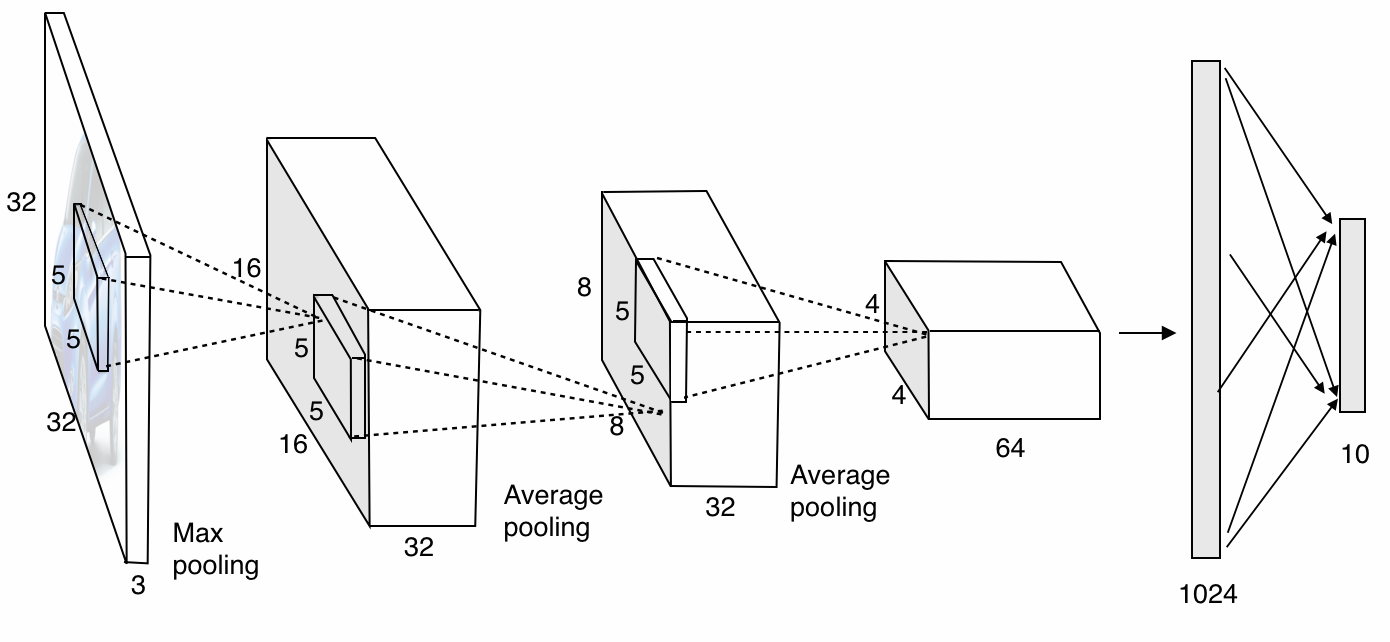
\includegraphics[width=1\textwidth]{architecture}
\caption{The architecture of our CNN.}
\label{fig1}
\end{figure}

\section{Sub-model Convolutional Network}
In this section, we start from introducing an effective technique called dropout. Inspired by dropout, we then introduce the concept of sub-model, and explore an improvement of network by linearly combining output of sub-models. We use convex optimization to find optimal weights of the combination.

\subsection{Dropout and sub-model combination}
Dropout is a recently-introduced technique to reduce overfitting \cite{imagenet}. It consists of setting to zero the output of each hidden neuron with probability of 0.5 in training procedure.  So every time a training example is presented, the neural network samples a different architecture, which we denote here as a sub-model $m_{k}$. All these sub-models share weights. At test time, we use all neurons but multiply their outputs by 0.5, which is an approximation to taking the geometric mean of the predictive distributions $P_{m_{k}}=\left [ P_{m_{k}}(Y=1),P_{m_{k}}(Y=2),...,P_{m_{k}}(Y=d) \right ]^{t}$ produced by the sub-models (where $d$ is the number of classes):

\begin{equation}
\begin{split}
\lim_{n\rightarrow \infty }(P_{m_{1}}(Y=i)\cdot P_{m_{2}}(Y=i)\cdot\cdot \cdot \cdot P_{m_{n}}(Y=i))^{\frac{1}{n}}&=\lim_{n\rightarrow \infty }(\frac{e^{(b_{i}+W_{i}\frac{1}{n}\sum_{k=1}^{n}h_{m_{k}})}}{(\sum_{j=1}^{d}e^{(nb_{j}+W_{j}\sum_{k=1}^{n}h_{m_{k}})})^{\frac{1}{n}}})
 \\
           &= \frac{e^{(b_{i}+W_{i}\cdot h_{comb})}}{\lim_{n\rightarrow \infty }(\sum_{j=1}^{d}e^{(nb_{j}+W_{j}\sum_{k=1}^{n}h_{m_{k}})})^{\frac{1}{n}}}
\end{split}
\end{equation}
\begin{equation}
P_{comb}(Y=i)=\frac{e^{b_{i}+W_{i}\cdot h_{comb}}}{\sum_{j=1}^{d}e^{b_{j}+W_{j}\cdot h_{comb}}}
\end{equation}



where $h_{m_{k}}$ is the neurons of the penultimate layer of sub-model $m_{k}$, and $h_{comb}$ is  that of the combined model by using all the neurons but multiply them by 0.5. $P_{comb}(\cdot)$ is the class membership probabilities of the combined model. 
\par
Apparently, the predictive distribution of the combined model is only a biased approximation of taking the mean of the predictive distribution of all sub-models.
\par
In our experiments (architecture shown in Figure~\ref{fig1}), dropout is performed in the output of penultimate layer, and $d=10$ is the number of classes of our dataset.
\par
Here, we want to explore a better option of combining the sub-models. Rather than giving an approximation, we want to actually take the linear combination of the predictive distribution of $n$ sub-models:
\begin{equation}
P_{l.comb}(Y=i) = \sum_{k=1}^{n}l_{k}\times P_{m_{k}}(Y=i)
\end{equation}
where $l_{k}$ is the weight of the distribution of $k$th model. The best weight $l=\left[ l_{1},l_{2}, ..., l_{n}\right]^{t}$ can be obtained by solving following optimization problem:
\begin{equation}
\begin{array}{rrclcl}
\displaystyle \min_{l} & \multicolumn{3}{l}{\sum_{i=1}^{N}\left \| P_{i}\cdot l-y_{i} \right \|_{2}^{2}}\\
\textrm{s.t.} & l& \succeq & 0\\
\end{array}
\end{equation}
\par
where $N$ is the number of all the training examples, $y_{i}$ is the $10 \times 1$ binary column vector indicating the true label of $i$th data point, and $P_{i} =\left [ P_{m_{1}},P_{m_{2}},...,P_{m_{n}} \right ] $ is a $10 \times n$ matrix, each column indicating the predictive probabilities of each sub-model. By minimizing the sum of squared l2 norm of difference between predicted distribution and true label, we find the non-negative weight vector $l$.
\par
The objective function can be simplified as following:
\begin{equation}
\begin{split}
\sum_{i=1}^{N}\left \| P_{i}\cdot l-y_{i} \right \|_{2}^{2} &=\sum_{i=1}^{N}(P_{i}\cdot l-y_{i})^{t}(P_{i}\cdot l-y_{i})
 \\
&=(P\cdot l-y)^{t}(P\cdot l-y)
 \\
&=l^{t}P^{t}Pl-2y^{t}Pl+y^{t}y
\end{split}
\end{equation}
where $y = \left[ y_{1}^{t}, y_{2}^{t},...y_{N}^{t}\right]^{t}$ is the concatenation of label indicator vectors of all data points, which is a $10N\times 1$ vector. $P = \left[ P_{1}^{t},P_{2}^{t},..., P_{N}^{t}\right]^{t}$ is the concatenation of probability distributions of all data points, which is a $10N \times n$  matrix. Then the optimization problem can be written as follow:
\begin{equation}
\begin{array}{rrclcl}
\displaystyle \min_{l} & \multicolumn{3}{l}{l^{t}P^{t}Pl-2y^{t}Pl+y^{t}y}\\
\textrm{s.t.} & l& \succeq & 0\\
\end{array}
\label{equation1}
\end{equation}
\par
This is a Quadratic Optimization Problem (QP), apparently a convex optimization problem, and is easy to solve.



\subsection{Sub-model combination in non-dropout CNN}
Now let's move back to CNN without dropout training. The same idea of sub-model combination can also be utilized to improve the performance of CNN when the network is trained without dropout. 
\par
The sub-models can be obtained by similar fashion with the dropout sub-models: given the already trained CNN model without dropout, randomly set penultimate units to zero with probability of 50\%, and multiply the remaining units by 2:
\begin{equation}
\textup{Pr}(h_{m_{i}}^{j}=2h_{orig}^{j})=\textup{Pr}(h_{m_{i}}^{j}=0)=\frac{1}{2}.
\end{equation}
where  $h_{m_{i}}$ is the 1024 penultimate-layer unit vector of the sub-model $m_{i}$, $h_{orig}$ is the 1024-unit vector of the trained CNN model, and $h_{(\cdot)}^{j}$ is the $j$th element of the vector. 
\par
Then, we can obtain the predictive distribution of each sub-model $P_{m_{k}}$, and the new model takes linear combination of the predictive distribution of $n$ sub-models, which is the same as the dropout condition:
\begin{equation}
P_{l.comb}(Y=i) = \sum_{k=1}^{n}l_{k}\times P_{m_{k}}(Y=i)
\end{equation}
\par
Therefore, the optimization problem is very similar with dropout condition (Equation~\ref{equation1}),  the only difference being the multiplication by 2 when obtaining the penultimate layer of sub-models.
\par
For both dropout network and non-dropout network, we expect improvement in performance on test set using a weighted combination of sub-models, when the number of sub-models used is large enough.

\section{Convex Loss functions}
Section 3 uses convex optimization for finding optimal combination of sub-models in CNN, while this section seeks to utilize convex optimization technique in deep learning from another perspective: focusing on alternatives of loss functions.
\par
Deep neural network is well-known for its high non-convexity. However, we can still borrow some ideas from the convex optimization literature\cite{svm}, where people have found many useful convex loss functions for classification tasks. In this section, we will talk about three different convex loss functions, and discuss how to use them in multiclass classification problem within the deep learning architecture.


\subsection{Cross-entropy}
Cross-entropy (CE) is the most standard loss function for neural networks, which is defined by:
\begin{equation}
H(p,q) = - \sum_{x}p(x)log q(x),
\end{equation}
where $p$ and $q$ are ground-truth posterior probability and estimated posterior probability respectively. Cross-entropy can be directly used for multiclass classification. This has been discussed in Section 2.1. 

\subsection{Hinge Loss}
Hinge loss is widely used in Support Vector Machines (SVMs). Given training data and its corresponding labels ($x_{n}$, $y_{n}$), $n=1,...,N$, $x_{n} \in R^{D}$, $t_{n} \in {-1,+1}$, for a binary classification problem, SVMs learning includes the following convex optimization:
\begin{equation}
\begin{array}{rrclcl}
\displaystyle \min_{w,\psi} & \multicolumn{3}{l}{ \frac{1}{2} w^{T}w +   C\sum_{n=1}^{N}\psi_{n}}\\
\textrm{s.t.} & w^{T}x_{n}t_{n}& \geq & 1-\psi_{n}  \forall n\\
&\psi_{n} & \geq 0& \forall n \\
\end{array}
\end{equation}

Hinge loss, while doesn't have a clear probability interpretation as CE, can be regarded as a maximum margin objective function, and it can be directly used in the deep learning architecture by deriving the corresponding unconstraint optimization problem:
\begin{equation}
\begin{array}{rrclcl}
\displaystyle \min_{w} & \multicolumn{3}{l}{ \frac{1}{2}w^{T}w+C\sum_{n=1}^{N}\textbf{max}(1-w^{T}x_{n}t_{n},0)}\\

\end{array}
\end{equation}

The second term of the object function is the Hinge loss. For the first term, there is a specific term called Weight Decay in the deep learning literature (which can also be seen as L2 regularization). The derivative w.r.t $x$ is:
\begin{equation}
\frac{\partial l(x)}{\partial x_{n}} = -Ct_{n}(\mathbb{I}(1>w^{T}x_{n}t_{n})),
\end{equation}
which is fast to compute.


Another similar loss function is the squared hinge loss:
\begin{equation}
\sum_{n=1}^{N}\textbf{max}(1-w^{T}x_{n}t_{n},0)^{2},
\end{equation}
which is also differentiable and easy to compute. It imposes a bigger loss for points which violate the margin.


To predict the class label, for a binary classification problem, it's simple:
\begin{equation}
\left\{\begin{matrix}
+1, if \, \, \, \, w^{T}x > 0\\
-1, \, \, \, \, otherwise 

\end{matrix}\right.
\end{equation}

\subsection{Multiclass Deep Neural Network with Hinge Loss}
Many methods have been proposed to generalize SVM to deal with multiclass problem. Here we talk about two most popular ways: One-Versus-All method and One-Versus-One method.

\subsubsection{One-Versus-All}
This is the earliest method for SVM multiclass classification. The basic idea is to train $K$ SVM models where $K$ is the number of classes. The $i$th SVM uses the data with label $i$ as the positive samples and the data with other labels as the negative samples. Interestingly, this idea can be easily implemented in deep learning architecture. We can have $K$ output units on top of the penultimate layer with the hinge loss. Then each output unit corresponds to one of
these One-Versus-All SVMs. We can also regard this as replacing the softmax and cross-entropy layer with the hinge loss layer. This kind of method works well for problem with a small number of classes. When the class number grows larger, the imbalance between positive and negative samples for each SVM becomes intolerable.

\subsubsection{One-Versus-One}
The One-Versus-One method is to construct $K(K-1)/2$ classifiers. Each is responsible for one of the $K(K-1)/2$ class pairs. While testing, we simply let all the binary classifiers vote for the most probable one, which is also called the ``Max Wins" strategy. To incorporate this method to deep learning architecture, we can have $K(K-1)/2$ output units, each of which corresponds to one classifier. All of the units use hinge loss. For each training data, only $K-1$ of these units
are activated. The other units are temperorily cut off. This is illustrated in Fig. \ref{mcsvm} 
\begin{figure}
\centering 
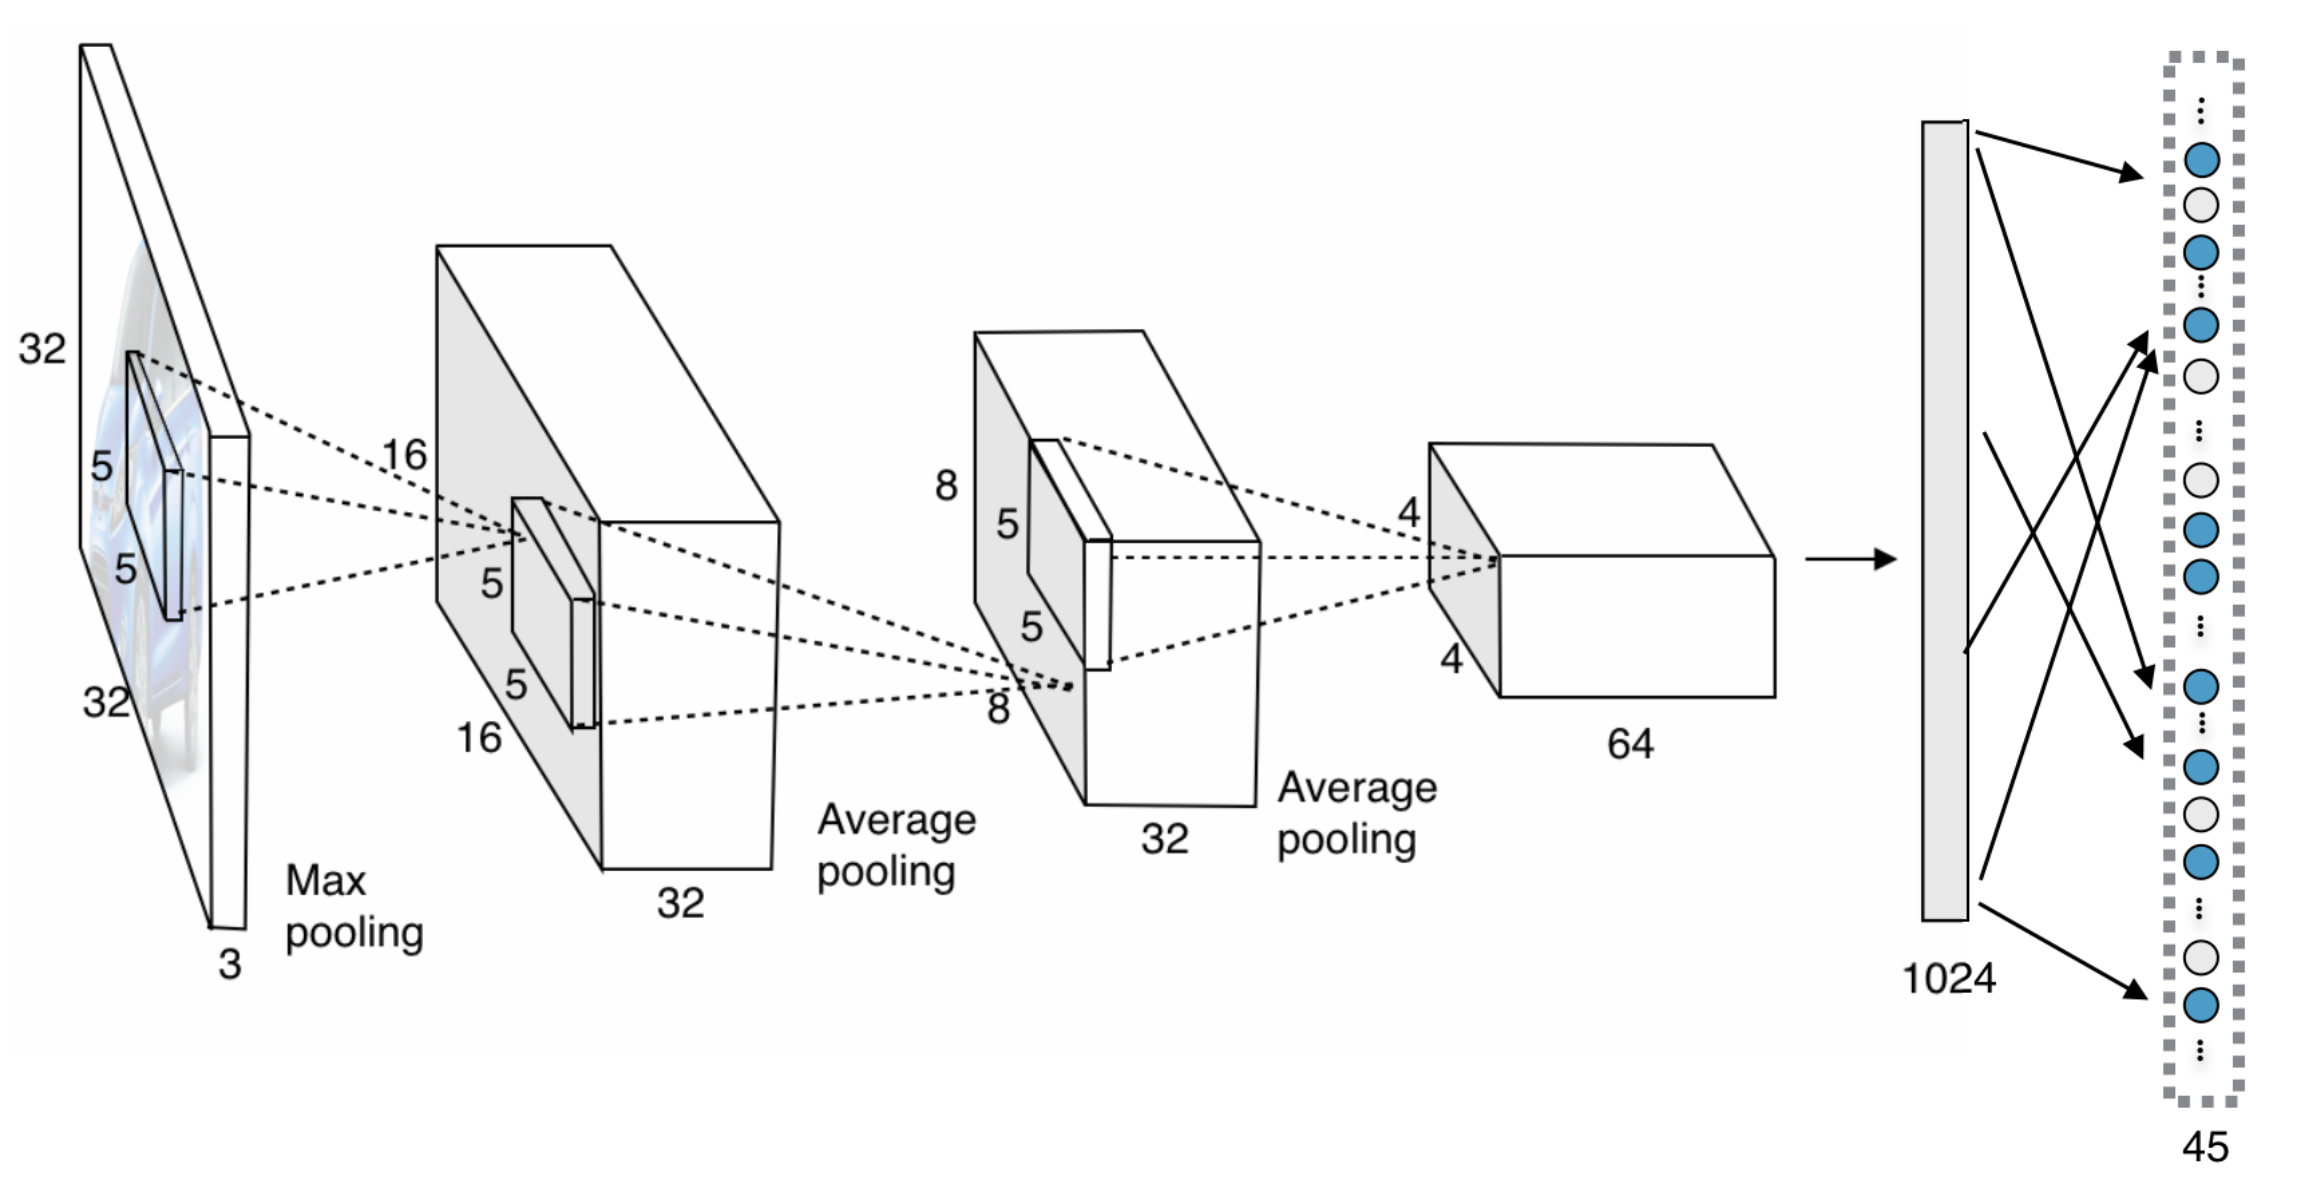
\includegraphics[width=0.8\textwidth]{MCSVM.png}
\caption{ Deep Neural Network with One-Versus-One Hinge Loss. Ultimate layer consists of $9\times 10/2=45$ units. For each training data, only 9 units (colored blue) are activated.}
\label{mcsvm} 
\end{figure}



The good property here is that for each SVM, the positive and negative training samples are balanced, no matter how many classes there are. However, the number of SVMs needed are quadratic in $K$, which makes it not scalable.

\subsection{Ranking Loss}
Another way to directly model the classification problem is the pairwise-ranking loss. Since we just want to pick the one with the highest linear output at test time. This leads to the following minimization problem:
\begin{equation}
\textup{Loss} = \sum_{n=1}^{N}\sum_{i \in C_{n}^{*}}\textbf{max}(0, 1-f_{j}(x_{n})+f_{i}(x_{n})),
\end{equation}
where $j$ is the label of the $n$th data and $C_{n}^{*}$ indicates the set of all the other labels. This loss can be directly generalized to multilabel predition problem and is widely used in many recommandation systems. 



\section{Experiments}
For all the experiments, the training and test data are CIFAR-10 dataset. There are 50,000 images in training set and 10,000 images in test set.
\subsection{Sub-model convolutional network}
In this section, we use Theano\cite{theano} to train and test the CNN model, and cvx toolbox\footnote{http://cvxr.com} in matlab to solve the convex optimization problem finding best weights. 
\subsubsection{Sub-model combination results}
We separately train the two networks with and without dropout, and the the results on the test set are shown in Table~\ref{table1}, this is the baseline of our experiments in this section.  For both networks, the learning rate is initialized to 0.001. Before reaching the final point, we decrease the learning rate twice(for each time we reduce it by a factor of 10).  Accuracy of dropout network is about 2\% higher than nondropout network, which shows the advantage of dropout method.
\par
Then, we randomly extract 4500 sub-models from dropout/non-dropout network respectively, and use different number of sub-models to obtain the combined model. For each combined model, we find the optimal weight $l$ by solving the convex optimization problem. The plot of the accuracy on test set versus number of sub-models is shown in Figure~\ref{accuracies}. The dotted line in both sub-figures are the accuracy of the original model, which is the approximation of geometric mean of all possible sub-models. We use this accuracy as a baseline.
\par 
For both networks, our sub-model CNNs outperform the original networks when the number of sub-models is large enough. Clearly, the accuracy tends to increase with the number of sub-models used. This is intuitive: the sub-models are chosen randomly; therefore the more sub-models we use, the more probable we have useful sub-models and better combinations. 
\par
There is one concern though: As is shown in Figure~\ref{accuracies}(a), for the network trained by dropout, the improvement is limited: the maximum accuracy achieved is 81.76\%, which is 0.22\% improvement from the baseline. On the other hand, for network trained without dropout, the improvement by weighted combination of sub-models is much more significant: the accuracy of original model is 79.52\%, and the weighed combination of sub-models is always much better than the original model, even when there are only 100 sub-models. The improvement is up to 0.76\% when the number of sub-models reaches to 3000. This is a non-trivial improvement from the original network.
\par
\begin{figure}
\centering 
\subfigure[Accuracy-number of sub-models for dropout network]{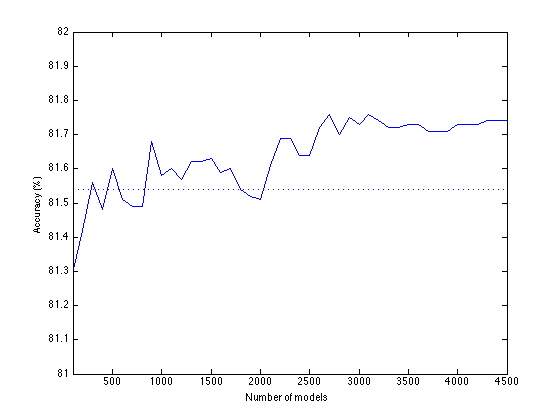
\includegraphics[width=0.8\textwidth]{dropout.png}} 
\subfigure[Accuracy v.s. number of sub-models for nondropout network]{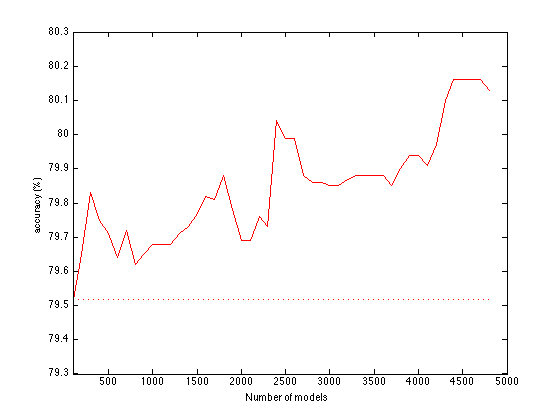
\includegraphics[width=0.8\textwidth]{nodropout.png}} 
\caption{ Accuracy v.s. number of sub-models.}
\label{accuracies} 
\end{figure}

\subsection{The role of dropout}
The reason of the lower improvement for dropout network is explained in this section. Dropout trains different sub-model at a time, but the weights are shared by all the sub-models. This procedure forces the network to learn more robust features that are useful for many different random sub-models, and after training, the sub-models in the dropout network can give similar results for all the data. This is the eventual goal of the dropout training. In other words, the sub-models in the dropout network are similar to each other, therefore whatever combination of them would not achieve much improvement. On the other hand, the network trained without dropout doesn't have the invariant property, thus the sub-models are quite different to each other, leading to greater improvement by combining them.
\par
Figure~\ref{hist} illustrates this invariance effect of dropout training more clearly. Accuracy achieved by each of 4500 sub-models for non-dropout/ dropout network is shown in the two histograms. Clearly, the sub-models of dropout network are much more concentrated than those of the non-dropout network. This shows the larger invariance of the sub-models in non-dropout network.
\begin{figure}
\centering 
\subfigure[Histogram of accuracies of sub-models of dropout network]{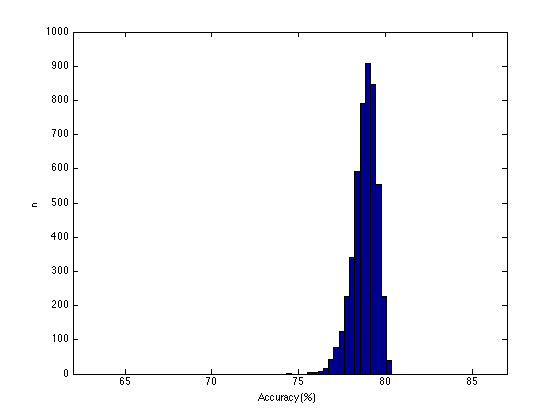
\includegraphics[width=0.8\textwidth]{dropout_hist.png}} 
\subfigure[Histogram of accuracies of sub-models of nondropout network]{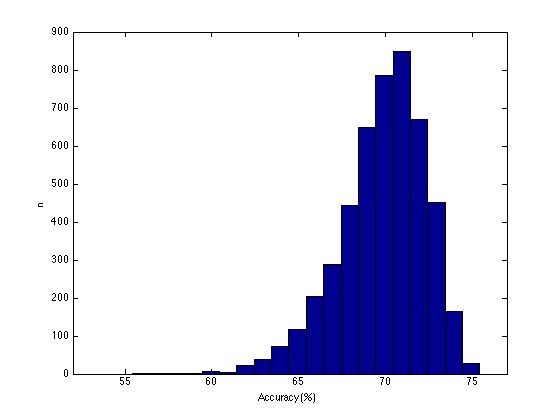
\includegraphics[width=0.8\textwidth]{nodropout_hist.png}} 
\caption{ Histograms of sub-models.}
\label{hist} 
\end{figure}

\begin{table}
\centering 
    \begin{tabular}{l|l}
    \hline
    Network     & Accuracy on test set (\%) \\ \hline
    Dropout     & 81.540                 \\ \hline
    Non-dropout & 79.517                 \\ \hline
    \end{tabular}
     \caption{Baseline: Accuracies of dropout/non-dropout networks}   
     \label{table1}
\end{table}

\subsection{Convolutional network with different convex loss functions}
For this part, we use Caffe to do the experiments. Caffe is the most popular and fastest deep convolutional network implementation for the time being. It provides the cross-entropy loss. For the other loss functions, we implemented by ourself. We are going to compare cross-entropy(CE), One-Versus-All hinge loss(1vsAll-L1), One-Versus-All square hinge loss(1vsALL-L2), One-Versus-One hinge loss(1vs1-L1), rank loss(RANK).
\subsubsection{Classification results}
\begin{table}
\centering 
    \begin{tabular}{l|l|l}
    \hline
    Loss     & Accuracy on test set (\%) & WeightDecay\\ \hline
    CE     & 77.85  &      750         \\ \hline
    1vsALL-L1 & 80.25  &   10            \\ \hline
    1vsALL-L2 &  80.18       &    100         \\ \hline
    1vs1-L1 &   77.80       &     10         \\ \hline
    RANK    &   77.60       &    100          \\ \hline
    \end{tabular}
     \caption{Accuracies with different loss functions and the corresponding weight decay}   
     \label{table2}
\end{table}
Table \ref{table2} shows the results for different loss functions and the corresponding relative weight decay used for the best results. For all of them, we use a similar strategy to train the network. The learning rate is initialized to 0.001. Before reaching the final point, we decrease the learning rate twice(for each time we reduce it by a factor of 10). The results clearly show that One-Versus-All hinge loss and square hinge loss outperform other methods by a large margin. Due to time limit, all the results shown above is the best from the parameters that we have
tried. 

\subsubsection{Convergence comparison}
We also plot the accuracy rate on the validation set for the first 50000 iterations while training(see Fig. \ref{conv}).
\begin{figure}
\centering 
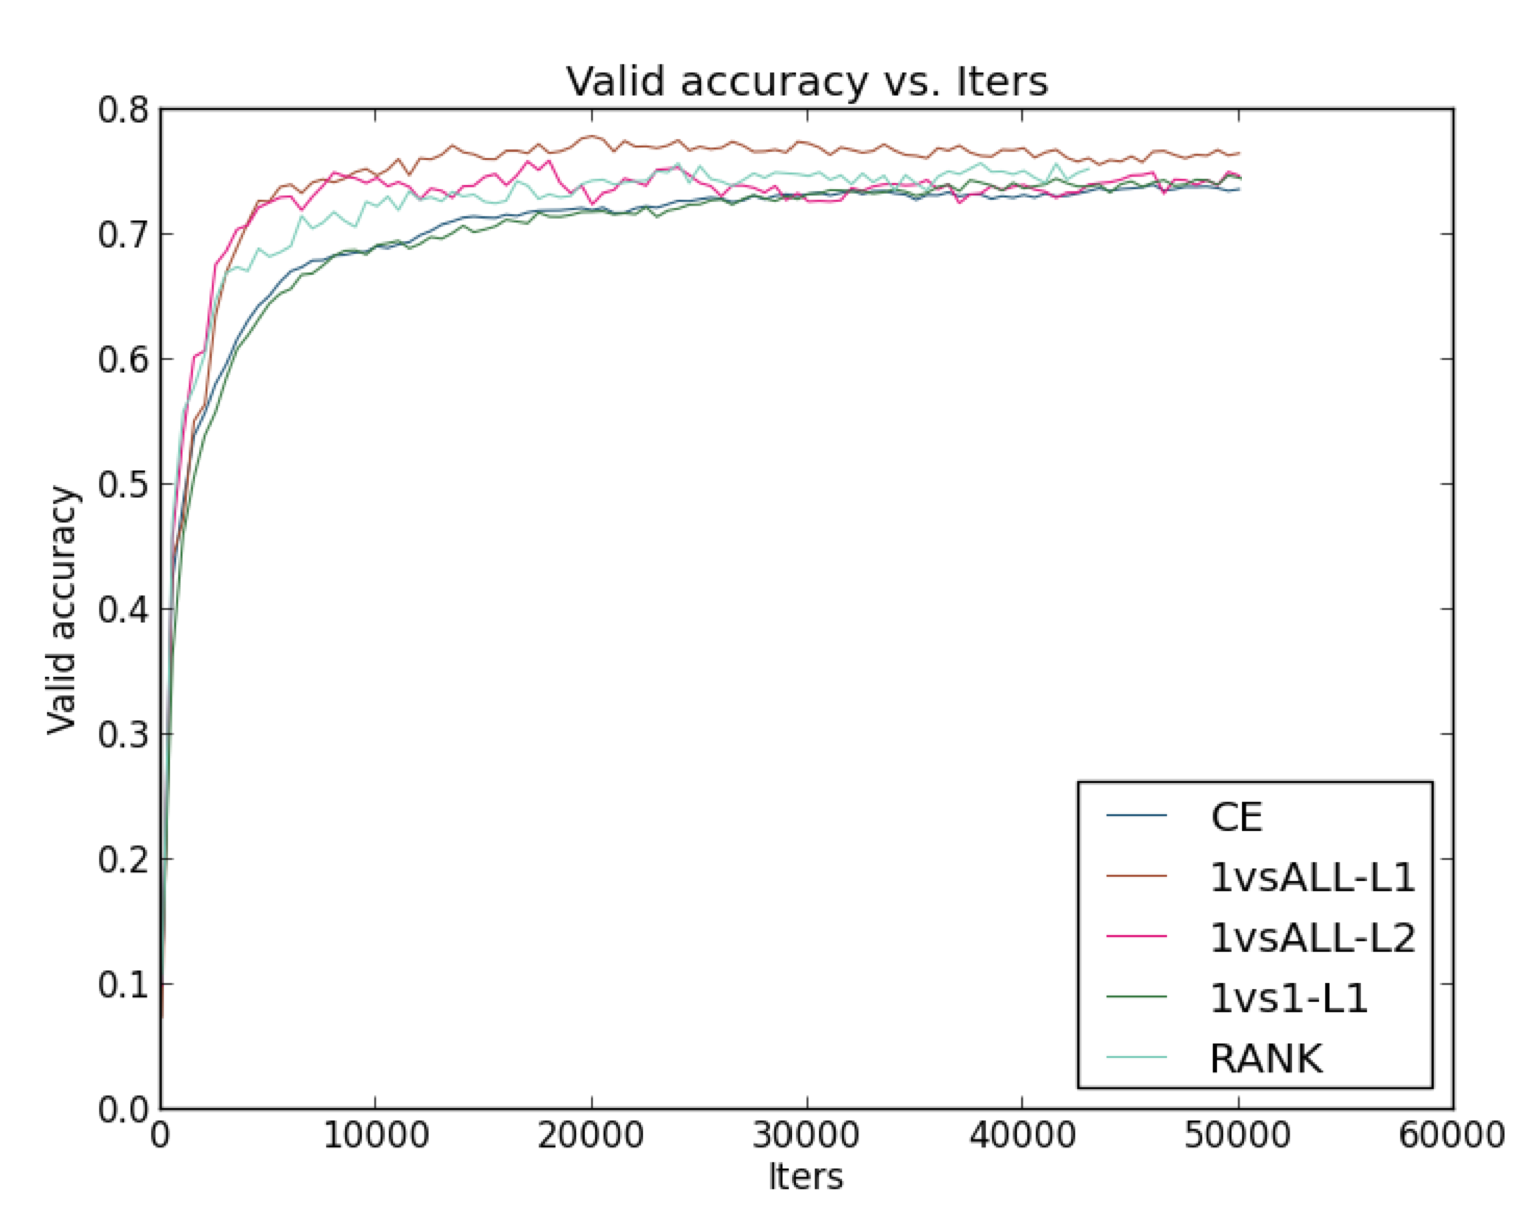
\includegraphics[width=0.8\textwidth]{plot_cnn.png}
\caption{Comparison for different loss functions while training}
\label{conv} 
\end{figure}
We can find that under the same learning rate(0.001), the One-Versus-All hinge loss and square hinge loss converge the fastest. Cross-entropy gives the smoothest curve.


Please note that even though in this dataset One-Versus-All hinge loss seems to outperform cross-entropy by a large margin, it doesn't mean that we can use them as the standard loss in the future. By some preliminary experiments, the One-Versus-All hinge loss doesn't work on CIFAR100, which is a 100 class extention of CIFAR10. Cross-entropy is standard because of its stability. Also, for One-Versus-One hinge loss and rank loss, we can not say for sure that they perform worse than
the others since the sets of parameters we have tried on them are too limited. This is why many people don't like neural networks. Tuning the parameters is a nightmare. However, we do find that by borrowing ideas from the convex optimization literature, we indeed see some improvements on some certain tasks. 



\section{Conclusion}
In this project, we explore two possible improvement of the Convolutional Neural Network architecture by using convex optimization methods:  1) Rather than taking the approximate geometric mean of the predictive distributions of all sub-models, we find an optimal linear combination of many sub-models. This modification improve the performance of both networks trained with and without dropout. We also discuss the role of dropout training in the formation of sub-models, and the reason why sub-model combination of dropout network yield less significant improvement; 2) We compare three different convex loss functions of the network, and provide our own implementation of utilizing these loss functions into multiclass classification problem.

\bibliographystyle{splncs}
\bibliography{ECE273}
\end{document}
